\documentclass[portuguese]{textolivre}

% metadata
\journalname{Texto Livre}
\thevolume{18}
%\thenumber{1} % old template
\theyear{2025}
\receiveddate{\DTMdisplaydate{2024}{9}{10}{-1}}
\accepteddate{\DTMdisplaydate{2025}{1}{7}{-1}}
\publisheddate{\today}
\corrauthor{Monalisa Pivetta da Silva}
\articledoi{10.1590/1983-3652.2025.54501}
%\articleid{NNNN} % if the article ID is not the last 5 numbers of its DOI, provide it using \articleid{} commmand 
% list of available sesscions in the journal: articles, dossier, reports, essays, reviews, interviews, editorial
\articlesessionname{articles}
\runningauthor{Silva e Minuzi}
%\editorname{Leonardo Araújo} % old template
\sectioneditorname{Daniervelin Pereira}
\layouteditorname{Leonardo Araújo}

%\usepackage{enumitem,longtable,array}
\usepackage{multirow}

\title{No rastro dos conceitos de competência digital docente}
\othertitle{In the wake of the concepts of teaching digital
competence}

\author[1]{Monalisa Pivetta da Silva~\orcid{0000-0002-1811-4044}\thanks{Email: \href{mailto:pesquisa.monalisa@gmail.com}{pesquisa.monalisa@gmail.com}}}
\author[2]{Nathalie Assunção Minuzi~\orcid{0000-0001-6465-7587}\thanks{Email: \href{mailto:nathalieminuzi@gmail.com}{nathalieminuzi@gmail.com}}}
\affil[1]{Universidade do Estado de Santa Catarina, 
Florianópolis, SC, Brasil.}
\affil[2]{Universidade Federal do Rio Grande do Sul, Porto Alegre, RS, Brasil.}

\addbibresource{article.bib}

\begin{document}
\maketitle
\begin{polyabstract}
\begin{abstract}
Este estudo é um recorte de uma tese de doutorado e tem
como objetivo explorar o conceito das competências digitais docentes.
Para tanto, foi realizada uma busca sistemática inspirada em métodos de
revisão integrativa, utilizando quatro bases de dados: \emph{Educational
Resources Information Center} (ERIC), \emph{Directory of Open Access
Journals} (DOAJ), \emph{Web of Science} (WoS) e \emph{Scopus
}(Elsevier). O problema de pesquisa questiona: o que são as competências
digitais docentes apresentadas nos estudos? O artigo identifica as
principais referências teóricas e documentais sobre o tema e destaca o
processo de seleção e classificação dos estudos selecionados. A análise
dos estudos selecionados foi conduzida por meio de um processo de
categorização e síntese das informações extraídas, considerando as
definições, abordagens e modelos teóricos adotados. Essas informações
podem contribuir para uma compreensão mais ampla das competências
digitais dos professores. Os resultados mostram que as competências
digitais dos professores são mais complexas do que as de outros
profissionais, exigindo uma formação específica que integre proficiência
tecnológica, compatibilidade pedagógica e consciência social. Conclui-se
que ser um professor digitalmente competente envolve não apenas
habilidades técnicas, mas também a capacidade de adaptar e aplicar essas
tecnologias de forma criativa e reflexiva no contexto educacional.

\keywords{Competência \sep Digital \sep Professor}
\end{abstract}

\begin{english}
\begin{abstract}
This study is an excerpt from a doctoral
thesis and aims to explore the concept of digital teaching skills. To
this end, a systematic search inspired by integrative review methods was
carried out, using four databases: \emph{Educational Resources
Information Center} (ERIC), \emph{Directory of Open Access Journals}
(DOAJ), \emph{Web of Science} (WoS), and \emph{Scopus }(Elsevier). The
research problem asks: what are the digital teaching skills presented in
the studies? The article identifies the main theoretical and documentary
references on the topic and highlights the selection and classification
process of the selected studies. The analysis of the selected studies
was conducted through a process of categorization and synthesis of the
information extracted, considering the definitions, approaches, and
theoretical models adopted. This information can contribute to a broader
understanding of teachers' digital skills. The results show that
teachers' digital skills are more complex than those of other
professionals, requiring specific training that integrates technological
proficiency, pedagogical compatibility, and social awareness. It is
concluded that being a digitally competent teacher involves not only
technical skills, but also the ability to adapt and apply these
technologies in a creative and reflective way in the educational
context.

\keywords{Competence \sep Digital \sep Teacher}
\end{abstract}
\end{english}
\end{polyabstract}

\section{Introdução}
O presente artigo é o recorte de uma tese de doutorado e apresenta o
conceito de competência digital docente, em uma busca sistemática
inspirada em métodos de revisão integrativa, realizada em quatro (4)
bases de dados: Educational Resources Information Center (ERIC),
Directory of Open Access Journals (DOAJ), Web of Science (WoS) e Scopus
(Elsevier). A questão central da pesquisa investiga como as competências
digitais docentes são definidas e caracterizadas nos estudos analisados
e tem como propósito analisar e aprofundar a compreensão do conceito de
competências digitais docentes.

Os artigos selecionados foram analisados com base em um processo de
categorização e síntese das informações, considerando as diferentes
definições, abordagens e modelos teóricos sobre competências digitais
docentes. A pesquisa identificou padrões e recorrências nos conceitos
apresentados, permitindo a organização dos principais elementos que
compõem essas competências.

As investigações e discussões em torno das temáticas das competências
digitais ganharam maior projeção nos últimos anos, refletindo sua
importância, especialmente no campo educacional. Diferentes organismos
internacionais
\cite{ocde2011, europeancommission2018}
têm manifestado interesse nessa área, com o desenvolvimento de programas
que envolvem padrões de referência para o desenvolvimento das
competências digitais e, em específico, as competências digitais dos
docentes.

O Brasil tem avançado na incorporação das competências digitais na
educação, impulsionado por políticas como a Política Nacional de
Educação Digital - PNED (2023), que promove a formação digital de
estudantes e professores. Em 2024, o Programa Nacional do Livro e do
Material Didático -- PNLD, incluiu a exigência de materiais digitais
interativos, e a Lei de Diretrizes e Bases da Educação Nacional reforçou
o letramento digital na educação básica e na formação docente.

O panorama contemporâneo da sociedade, permeado pela presença
onipresente das tecnologias da informação e comunicação (TICs), demanda
uma compreensão profunda e atualizada do conceito de competência
digital. Essa noção, amplamente discutida na literatura acadêmica,
revela-se como um constructo multifacetado, dinâmico e em constante
evolução \cite{ferrari2013}. É nesse contexto que se insere a presente
pesquisa, visando elucidar os principais pontos conceituais e suas
implicações para a prática docente.

Em termos gerais, a mobilização de competências digitais implica
conhecer e utilizar as tecnologias com criticidade e responsabilidade,
consideradas indispensáveis para o desenvolvimento da cidadania em uma
sociedade digital.

O conceito de competência digital abrange a habilidade técnica, mas
também a capacidade de enfrentar novos desafios tecnológicos de forma
flexível. Isso implica na análise crítica de informações, e o
aproveitamento do potencial tecnológico para promover a colaboração e
construção de conhecimento compartilhado, ao mesmo tempo que se
desenvolve a consciência das responsabilidades pessoais e o respeito
pelos direitos e deveres.

Entende-se que o contexto das competências digitais docentes vai além da
mera habilidade técnica; requer uma conscientização ampla sobre o uso
ético e eficaz da tecnologia para promover a aprendizagem e a segurança
dos alunos.

Neste artigo apresentam-se os resultados de como os conceitos de
competência digital docente são acordados nas pesquisas, identificando
as principais referências e bases teóricas. Destaca-se o processo de
busca, seleção e classificação dos artigos, a análise dos estudos
selecionados e sua distribuição geográfica, bem como a importância das
referências e documentos oficiais no campo.



\section{Conceitos de Competências Digitais}
O conceito de competência digital é amplo, multidimensional, complexo e
dinâmico. Considerando tais características é preciso considerar os
múltiplos olhares sobre esse tema. Conforme \textcite{silva2019a} indicam
que inicialmente, era utilizado o termo letramento digital com é a
capacidade de ler, escrever e interpretar conteúdos digitais, utilizando
dispositivos como computadores, celulares e tablets. A \emph{posteriori,
}o letramento digital foi incorporado no marco europeu de CD (2006) como
um nível para ser desenvolvido junto aos sujeitos.

Além desse termo, também alguns autores tratam a alfabetização digital e
letramento digital como sinônimos. No entanto, \textcite{silva2019a}
abordam que ``supõe aceitar, com todas as suas consequências, que as
aprendizagens relacionadas com o domínio e manejo das TDICs são básicas
na SI.'' \cite[s.p.]{silva2019a}

Dessa forma, as competências digitais consistem numa série de áreas de
conhecimento e estão em constante construção, uma vez que tendem a
acompanhar a evolução das tecnologias e a sua utilização na sociedade
\cite{ferrari2013}.

\textcite[p.~186]{calvani2009} descrevem a competência digital
como a capacidade de:
\begin{quote}
explorar e enfrentar as novas situações tecnológicas de uma maneira
flexível para analisar, selecionar, avaliar criticamente os dados e
informações, aproveitando o potencial tecnológico para representar,
resolver problemas, construir conhecimento compartilhado e colaborativo,
enquanto se fomenta a consciência de suas próprias responsabilidades
pessoais e o respeito recíproco dos direitos e obrigações. (tradução
nossa).
\end{quote}

Com o objetivo de identificar como as pesquisas abordam este tema,
\textcite{ferrari2012} foi utilizada como marco teórico, uma vez que o conceito
elaborado por ela é o mais utilizado nas definições de competências
digitais:
\begin{quote}
{[}...{]} o conjunto de conhecimentos, aptidões, atitudes, habilidades,
estratégias e consciência que são necessários na utilização das TIC's
{[}tecnologias da informação e da comunicação{]} e meios digitais, para
executar tarefas; resolver problemas; comunicar; gerenciar informação;
colaborar; criar e compartilhar conteúdos; e construir conhecimentos de
forma eficaz de forma eficiente, apropriada, crítica, criativa,
autônoma, flexível, ética, reflexiva para o trabalho, lazer,
participação, aprendizagem, socialização e empoderamento \cite[p.~3-4, tradução nossa]{ferrari2012}.
\end{quote}

\textcite{ferrari2012} se destaca como uma das principais referências do
conceito de competência digital, ao definir como um conjunto abrangente
de conhecimentos, habilidades, atitudes e estratégias necessárias para a
utilização eficaz das TICs e mídias digitais em uma variedade de
contextos. Tal definição abarca desde a execução de tarefas cotidianas
até a construção de conhecimento de forma autônoma e reflexiva.

Entretanto, evidencia-se que nem sempre há um consenso sobre a
conceituação da competência digital. De acordo com os estudos de \textcite{silva2019a} os termos ligados a \emph{Literacy }(Letramento), como
\emph{Technology Literacy} ou \emph{Technological Literacy} (Letramento
Tecnológico), \emph{New Literacies} (Novos Letramentos), \emph{ICT
Literacy} (Letramento em TIC), \emph{Media Literacy} (Letramento em
Mídias), \emph{eLiteracy} (eLetramentos), encontram-se na mesma linha do
conceito de \emph{Digital Literacy.}

\textcite{redecker2012} consideram o letramento digital algo
mais do que uma habilidade técnica para operar adequadamente com
dispositivos digitais. Para eles trata-se da combinação de um conjunto
de competências técnico-processuais, cognitivas e socioemocionais,
necessárias para viver, aprender e trabalhar em uma sociedade digital.

Esses autores consideram que os conceitos de alfabetização digital e
competência digital têm diferentes conotações e diferentes
interpretações, sendo a competência digital a soma de múltiplos
letramentos: tecnológico, informacional, audiovisual e comunicativo;
além de ser um novo letramento que implica novos componentes e maior
complexidade \cite{ferrari2012}.

É importante uma abordagem que vai além do domínio técnico, englobando
aspectos informacionais, multimídia e comunicativos. Nessa perspectiva,
\textcite{gewerc2015} destacam a necessidade de desenvolver
habilidades para comunicar, interpretar e produzir mensagens em
diferentes mídias, promovendo a autonomia e o espírito crítico além de
facilitar a transferência de conhecimento para diferentes contextos, por
meio de dispositivos tecnológicos para resolver problemas reais
\cite{gewerc2015}. A competência digital não implica apenas a posse de
tais habilidades, conhecimentos e atitudes, mas a capacidade de
colocá-los em ação, mobilizá-los, combiná-los e transferi-los para agir
de forma consciente e eficaz para um propósito.

As definições mencionadas ilustram a complexidade do conceito ao indicar
que o desenvolvimento da competência digital envolve mais do que
competências técnicas e vai além de tratar a informação e transformá-la
em conhecimento.

A análise das contribuições de diversos estudiosos revela uma
convergência de aspectos fundamentais. Ao analisar os conceitos, \textcite{silva2022} compreende a competência digital como:
\begin{quote}
a utilização consciente e crítica das tecnologias digitais, na
mobilização de habilidades que permitem buscar, selecionar e processar a
informação; capacidade de se comunicar usando diferentes suportes
tecnológicos e digitais para informar-se colaborar, criar, compartilhar
conteúdos, aprender, socializar e resolver problemas, atuando com
responsabilidade e ética. \cite[p.~57]{silva2022}
\end{quote}

O desenvolvimento de competências digitais é essencial para a inclusão
na sociedade digital, na qual os avanços tecnológicos ocorrem
rapidamente, de acordo com \textcite{escudero2019}. Assim,
verifica-se que a competência digital dos professores tem sido objeto de
diversas pesquisas e de documentos orientadores, dada a necessidade de
educar as futuras gerações em uma sociedade em constante mudança.

Considerando esse cenário de transformação, o estudo visa compreender de
que modo as pesquisas sobre competências digitais estão abordando isso
com os docentes. Para tanto, a seguinte seção apresenta a metodologia
baseada em uma busca sistemática para identificar o conceito
``competências digitais docentes''.



\section{Metodologia: Busca sistemática acerca das competências
digitais docentes}

A busca sistemática apresentada neste artigo utilizou elementos da
revisão integrativa, baseada nos métodos sistemáticos e explícitos para
identificar, selecionar e avaliar criticamente pesquisas relevantes e
analisar os dados de estudos. De acordo com \textcite{mendes2008}, uma revisão integrativa segue algumas etapas: 1) preparação da
pergunta da revisão; 2) busca e seleção dos estudos primários; 3)
extração de dados dos estudos; 4) avaliação crítica dos estudos
primários incluídos na revisão; 5) síntese dos resultados da revisão; e
6) apresentação do método \cite{mendes2008}.

Desse modo, procurou-se compreender as concepções de competências
digitais docentes nas pesquisas analisadas. A fim de elucidar o conceito
a busca sistemática foi organizada conforme as etapas sugeridas por
\textcite{galvao2014} apresentadas na \Cref{tab01}.

\begin{table}[htbp]
\centering
\begin{threeparttable}
    \caption{Etapas da busca sistemática}
    \label{tab01}
    \begin{tabular}{l p{0.8\textwidth}}
    \toprule
      1a etapa & Traçar objetivo, definir a questão da pesquisa e identificar as palavras-chave. \\
      2a etapa & Estabelecer critérios de inclusão e exclusão; uso de base de dados; e seleção dos estudos. \\
      3a etapa & Extrair as informações; organizar e sumarizar as informações; e formar o banco de dados. \\
      4a etapa & Avaliar a inclusão/exclusão de estudos. \\
      5a etapa & Analisar criticamente os estudos selecionados e discutir os resultados. \\
      6a etapa & Sintetizar o conhecimento ou as informações obtidas. \\
    \bottomrule
    \end{tabular}
    \source{elaborado com base em \textcite{mendes2008}.}
\end{threeparttable}
\end{table}

Com o objetivo de traçar um panorama acerca das competências digitais e
das competências digitais docentes, foi considerado o período entre 2013
e 2021. Assim, foi realizada busca sistemática partindo da questão
direcionadora: quais os conceitos de competências digitais docentes
apresentados nos artigos?


Quanto aos critérios de seleção das pesquisas, foram definidos os
seguintes filtros:
\begin{enumerate}[label=\alph*)]
    \item estudos publicados entre 2013 e 2021;
    \item área: educação;
    \item idiomas: português, inglês e espanhol;
    \item tipo de documento: pesquisas primárias (artigo de periódico);
    \item artigos abertos ao público.
\end{enumerate}

A busca dos artigos foi realizada em quatro bases de dados, da área da
educação e multidisciplinares: \emph{Educational Resources Information
Center} (ERIC), \emph{Directory of Open Access Journals} (DOAJ),
\emph{Web of Science} (WoS) e \emph{Scopus }(Elsevier).

Após a definição das bases de dados, foi construída a String de busca
para ser utilizada nas bases. Assim foram consideradas as seguintes
String:("Digital competence" OR "Digital literacy" OR "Digital skills")
AND Teacher) AND Education). Os termos em inglês e espanhol foram
utilizados para dar maior amplitude à busca de pesquisas.

Os termos da busca derivam do uso de termos frequentemente utilizados em
pesquisas relacionadas à competência digital em educação. Do resultado
dessa busca, examinamos as referências mais utilizadas e partimos para a
reflexão do que são as competências digitais docentes e como são
abordadas pelos autores e pelos documentos e recomendações
internacionais citados nas pesquisas.




\section{Resultados e discussão: Análise dos estudos
selecionados}

A partir dos critérios e filtros aplicados, foram identificados 672
artigos (na primeira busca) e 486 artigos na segunda busca (atualização)
que continham os termos ``competências digitais'' citados no título,
resumo ou palavras-chave, totalizando 1158 artigos. A base de dados
\emph{Web of Science} apresentou algumas variações. Por exemplo, na
falta de um filtro específico para a área da Educação, foi utilizado o
filtro pela área de conhecimento ``\emph{Social Sciences}'', que abarcou
mais resultados da temática pretendida. Para limitar a busca, aplicou-se
ainda o filtro das palavras-chave. Os dados foram selecionados e
exportados para um equipamento no formato .csv e organizados por ano e
base, incorporando código alfanumérico único para cada artigo.


\begin{table}[htbp]
\centering
\begin{threeparttable}
    \caption{Número de artigos por ano nas bases}
    \label{tab02}
    \begin{tabular}{lllllll}
    \toprule
    Ano & ERIC\tnote{1} & DOAJ\tnote{2} & WOS\tnote{3} & Scopus & Total & \% \\
    \midrule
2013 & 06 & 01 & 06 & 21 & 34 & 3\% \\
2014 & 14 & 00 & 02 & 20 & 36 & 3\% \\
2015 & 12 & 00 & 30 & 38 & 80 & 7\% \\
2016 & 11 & 05 & 50 & 36 & 102 & 9\% \\
2017 & 24 & 03 & 42 & 49 & 118 & 10\% \\
2018 & 14 & 03 & 45 & 74 & 136 & 12\% \\
2019 & 10 & 02 & 73 & 81 & 166 & 14\% \\
2020 & 98 & 04 & 93 & 87 & 282 & 24\% \\
2021 & 54 & 02 & 83 & 65 & 204 & 18\% \\
Total & 243 & 20 & 424 & 471 & 1158 & 100\% \\
    \bottomrule
    \end{tabular}
    \begin{tablenotes}
    \item[1] Education Resources Information Center;
    \item[2] Directory of Open Access Journals;
    \item[3] Web of Science; 
    \end{tablenotes}
    \source{\textcite{silva2022}.}
\end{threeparttable}
\end{table}

A partir da organização da \cref{tab02}, observou-se um crescimento
significativo nas pesquisas relacionadas a competências digitais ao
longo dos anos. Em 2013, foram encontrados 34 artigos, e em 2020 esse
número aumentou para 282 artigos, em relação à pesquisa realizada nas
bases com os filtros selecionados.

\textcite{rodriguezgarcia2019} destacam que essa
temática se posiciona como um dos tópicos mais relevantes no campo da
tecnologia e seu impacto na sociedade atual. Neste estudo, a análise
envolveu a exclusão de artigos repetidos e a classificação dos restantes
com base em sua temática principal. Dos 1158 artigos inicialmente
analisados, 130 foram excluídos por serem repetidos não privilegiando
nenhuma base de dados específica. Os 1027 restantes foram então
classificados, e 186 deles, que tinham "competência digital" como tema
central, em que o termo competência digital constava no título, foram
selecionados.

Após a leitura dos resumos, foram excluídos os artigos que não tinham
relação direta com o contexto educacional, restando assim 77 artigos.
Esses foram categorizados e lidos na íntegra e optou-se por excluir os
artigos que os sujeitos das pesquisas se referiam a professores do
ensino superior, mantendo apenas as pesquisas em que os sujeitos eram
professores da educação básica de ensino. Assim, foram selecionados 30
artigos que cumpriam todos os critérios para a análise e discussão dos
resultados. Desses artigos, vinte pertenciam à base \emph{Web of
Science}, sete pertenciam à base \emph{Eric }e três à base
\emph{Scopus}. Verifica-se uma síntese desse processo na \cref{fig01}.

\begin{figure}
    \centering
    \begin{minipage}{0.75\linewidth}
    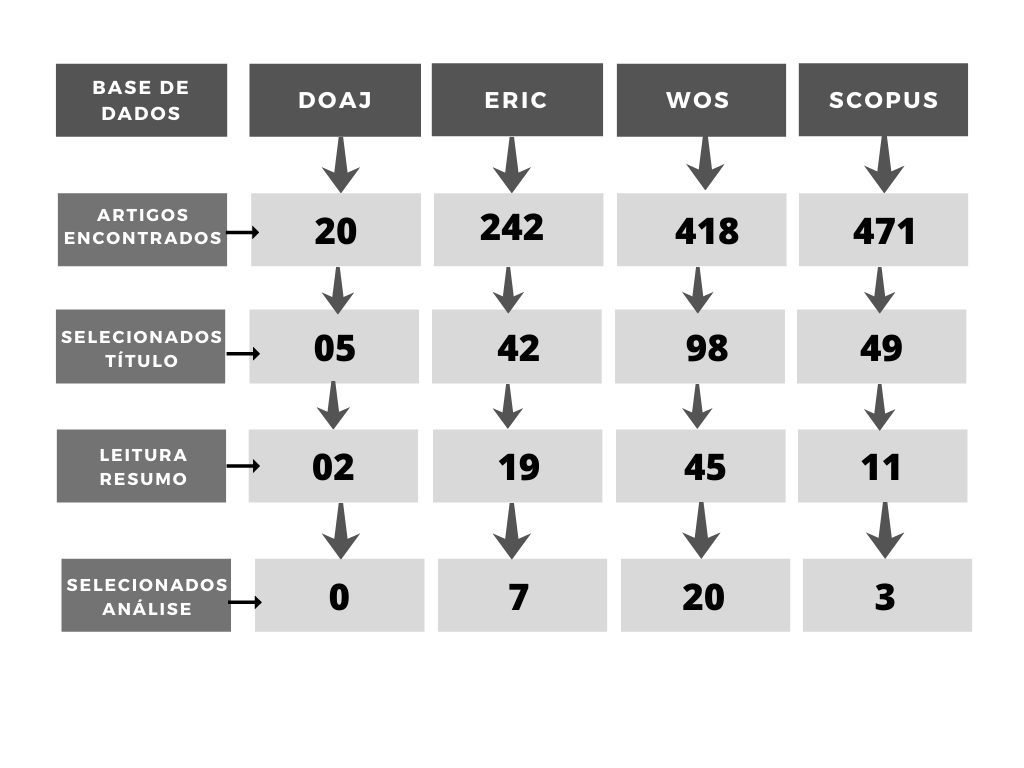
\includegraphics[width=\linewidth]{figure01.png}
    \caption{Fluxograma com a sequência da busca sistemática}
    \label{fig01}
    \source{\textcite{silva2022}}
    \end{minipage}
\end{figure}

Para a análise dos estudos selecionados, identificaram-se os conceitos
de competência digital docente abordados (a definição utilizada pelos
autores), bem como as bases teóricas que fundamentam a discussão da
temática. A partir dos critérios estabelecidos, elaborou-se o quadro
síntese com os artigos selecionados:

\begin{footnotesize}
\renewcommand{\arraystretch}{1.5}
\begin{longtable}{
    @{}l >{\raggedright\arraybackslash}p{0.66\textwidth}
    ll
    >{\raggedright\arraybackslash}p{0.15\textwidth}@{}
    }
\caption{Artigos selecionados na revisão}
\label{tbl02}
\\
\toprule
	& Título & Ano & Base & Autores \\
\midrule
1 & Aligning teacher competence frameworks to 21st century challenges: The case for the European Digital Competence Framework for Educators (DIGCOMPEDU) \newline
Alinhando os quadros de competência dos professores aos desafios do século XXI: O caso do Quadro Europeu de Competências Digitais para Educadores (DIGCOMPEDU) & 2019 & WOS & Caena, F; Redecker, C \\
2 & Análisis de la autopercepción sobre el nivel de competencia digital docente en la formación inicial de maestros/as. \newline
Análise da autopercepção sobre o nível de competência digital dos professores na formação inicial & 2019 & WOS	& Escudero, VG; Gutierrez, RC; Somoza, J.A.G.C \\
3 &	Appropriation of digital competence in teacher education \newline
Apropriação da competência digital na formação de professores & 2014 & WOS & Instefjord, E \\
4 & Development of digital competence in secondary education teachers’ training \newline
Desenvolvimento da competência digital na formação de professores do ensino secundário & 2018 & SCO & Fraile M.N., Peñalva-Vélez A., Lacambra A.M.M. \\
5 & Desarrollo de la competencia digital en la formación inicial del profesorado de educación infantil \newline 
Desenvolvimento da competência digital na formação inicial de professores da educação infantil & 2018 & SCO & Llorente P.A., Iglesias E.C. \\
6 & Digital Storytelling: Activating communicative, narrative and digital competences in initial teacher training. \newline 
Digital Storytelling: Ativação de competências comunicativas, narrativas e digitais na formação inicial de professores & 2016 & WOS & Del Moral, ME; Villalustre, L; 
Neira, MD \\
7 & Educating teachers for the new millennium? Teacher training, ICT and digital competence \newline
Educando professores para o novo milênio? Formação de professores, TIC e Competência digital & 2015 & WOS & Tømte, CE \\
8 & ETeach3D: Designing a 3D virtual environment for evaluating the digital competence of preservice teachers \newline
ETeach3D: Projetando um ambiente virtual 3D para avaliar a competência digital dos futuros professores & 2016 & WOS & Esteve-Mon, FM; Cela-Ranilla, JM; Gisbert-Cervera, M\\
9 & Evaluation and development of digital competence in future primary school teachers at the University of Murcia \newline
Avaliação e desenvolvimento da competência digital nos futuros professores do ensino primário da Universidade de Múrcia & 2016 & WOS & Porlan, IG; Sanchez, JLS\\
10 & La competencia digital de los futuros docentes: ¿cómo se ven los actuales estudiantes de Educación? \newline
A competência digital dos futuros professores: qual é a percepção dos atuais estudantes de Educação?	& 2016 & WOS & Esteve-Mon, F.M; Gisbert-Cervera, M; Lazaro-Cantabrana, JL \\
11 & Indicadores para evaluar la competencia digital docente en la formación inicial en el contexto Chileno – Uruguayo. \newline
Indicadores para avaliar a competência digital de professores em formação inicial no contexto Chile – Uruguai & 2016 & WOS & Quiroz, JS; Miranda, P; Gisbert, M; Morales, J; Onetto, A \\
12 & Alfabetización informacional y competencia digital en estudiantes de magisterio \newline
Literacia informativa e competência digital em estudantes do magistério & 2018 & WOS & Rodríguez, MDM; Mendez, VG; Martin, AMR \\
13 & Maltese Primary Teachers'Digital Competence: Implications for Continuing Professional Development \newline
Competência digital dos professores primários malteses: Implicações para o desenvolvimento profissional contínuo & 2017 & ERIC & Spiteri, M.; Chang Rundgren, S.\\
14 & On the Issues of Digital Competence in Educational Contexts - A Review of Literature \newline
Sobre as Questões de Competência Digital em Contextos Educacionais- Uma Revisão da Literatura & 2018 & ERIC & Pettersson, F. \\
15 & Percepción de estudiantes de Pedagogía sobre el desarrollo de su competencia digital a lo largo de su proceso formativo \newline
Percepção de alunos de Pedagogia sobre o desenvolvimento de sua competência digital ao longo de seu processo formativo & 2016 & SCO	& Flores-Lueg C., Vila R.R.\\
16 & Prepared to teach ESL with ICT? A study of digital competence in Norwegian teacher education \newline
Preparado para ensinar segunda língua com TIC? Um estudo de competência digital na formação de professores noruegueses & 2016 & WOS & Røkenes, FM; Krumsvik, RJ \\
17 & Preparing pre-service teachers to integrate technology: an analysis of the emphasis on digital competence in teacher education curricular \newline
Preparação dos futuros professores para integrar a tecnologia: uma análise da ênfase na competência digital nos currículos de formação de professores & 2016 & WOS & Instefjord, E; Munthe, E \\
18 & Conocimiento profesional y competencia digital en la formación del profesorado. El caso del Grado de Maestro en Educación Primaria \newline
Conhecimento profissional e competência digital na formação de professores. O caso da formação de professores do ensino básico & 2015 & WOS & Gewerc, A; Montero, L \\
19 & Teacher's digital competence among final year pedagogy students in Chile and Uruguay \newline 
Competência digital docente entre alunos do último ano de pedagogia no Chile e no Uruguai	& 2019 & WOS & Silva, J; Usart, M; Lazaro-Cantabrana, J.L \\
20 & The Development of Digital Competence of Students of Teacher Training Studies-Polish Cases \newline
O Desenvolvimento da competência digital dos estudantes da formação de professores - Casos Polacos & 2019 & ERIC & Nowak, B. M. \\
21 & El desarrollo de la competencia digital docente a partir de una experiencia piloto de formación en alternancia en el Grado de Educación \newline
O desenvolvimento da competência digital docente a partir de uma experiência-piloto de formação em alternância no âmbito da licenciatura em Educação & 2015 & WOS & Cantabrana, J.L; Cervera, M. G \\
22 & A study of the use of digital technology and its conditions with a view to understanding what ‘adequate digital competence’ may mean in a national policy initiative \newline
Um estudo sobre o uso da tecnologia digital e suas condições com vistas a entender o que a "competência digital adequada"pode significar em uma iniciativa de política nacional & 2020 & ERIC & Olofsson, A D; Fransson, G; Lindberg, J.O \\
23 & A Study on the Actual Use of Digital Competence in the Practicum of Education Degree \newline
Estudo sobre o uso real da Competência Digital na prática do curso de Educação [licenciatura] & 2020 & ERIC & Gámez, F.D.G. Fernández, M.J.M.; García, F.J.A. \\
24 & Analysis of digital competence of educators (DigCompEdu) in teacher trainees: the context of Melilla, Spain \newline
Análise da competência digital dos educadores (DigCompEdu) em professores estagiários: o contexto de Melilla, Espanha & 2021 & WOS & García, J.M.G.V; García -Carmona, M.; Torres, JMT; Fernandez, P.M. \\
25 & ¿Estamos técnicamente preparados para el flipped classroom? Un análisis de las competencias digitales de los profesores en España \newline
Estamos tecnicamente prontos para a sala de aula invertida? Uma análise das competências digitais de professores na Espanha & 2020 & WOS & Celaya, LAA; Campión, RS; Eguizabal, JMS \\
26 & Comparative research in the digital competence of the pre-service education teacher: face-to-face vs blended education and gender \newline
Pesquisa comparativa na competência digital do professor de educação inicial: educação presencial vs educação mista e gênero & 2020 & WOS	& Guillen Gamez, F.D.G.; Mayorga Fernández, M.J.; Del Moral, MT \\
27 & Competencias digitales y resiliencia: una revisión teórica enfocada en el profesorado \newline
Competências digitais e resiliência: uma revisão teórica focada em professores & 2021 & WOS & Holguin- Alvarez, J.; Rodríguez Rojas, M.; Romero Hermoza, R.M.; Perez, F.L.; Cruz Montero, J. \\
28 & Exploring the digital competence of pre-service teachers on entry onto an initial teacher education programme in Ireland \newline
Explorando a competência digital de estudantes em um programa inicial de formação de professores na Irlanda & 2021 & ERIC & McGarr, O.; McDonagh, A. \\
29 & From digital literacy to digital competence: the teacher digital competency (TDC) framework \newline
Da alfabetização digital à competência digital: a estrutura de competência digital do professor (TDC) & 2020 & ERIC & Falloon, G. \\
30 & The ethical dimension of digital competence in teacher training \newline
A dimensão ética da competência digital na formação de professores & 2021 & WOS & Novella García, C. N; Lozano, A. C. \\
\bottomrule
\source{\textcite{silva2022}.}
\end{longtable}
\end{footnotesize}

A análise dos 30 artigos selecionados revelou aspectos relacionados às
competências digitais dos professores. Esses artigos foram categorizados
com base em seus objetivos, que abrangem a avaliação do nível de
competência digital, estratégias e formas para desenvolver as
competências digitais, análise de documentos e currículos e criação de
instrumentos e ambientes para sua avaliação. A maioria dos artigos se
concentra na formação e cursos de professores, bem como na avaliação do
nível de competência digital dos mesmos.

Na \Cref{tbl03}, são apresentados os objetivos dos artigos agrupados por
categorias:

%
%
% TABELA
%
\begin{footnotesize}
\renewcommand{\arraystretch}{1.5}
\begin{longtable}{
    >{\raggedright\arraybackslash}p{0.2\textwidth}
    >{\raggedright\arraybackslash}p{0.75\textwidth}
    }
\caption{Categorias e objetivos dos artigos}
\label{tbl03}
\\
\toprule
Categorias & Objetivos dos artigos \\
\midrule
\multirow[t]{6}{=}{CD apresentada em quadros de referência e investigações} & A1 – Apresentar o marco europeu para competência digital dos professores \\
									    & A13 – Investigar a competência digital dos professores malteses e recomendar formação para integração tecnológica nas práticas de ensino\\
									    & A14 – Examinar como os aspectos pedagógicos da competência digital são abordados nas investigações internacionais ao longo dos últimos 10 anos.\\
									    & A20 – Apresentar as várias áreas de debate em relação às competências digitais e as necessidades educativas atuais.\\
									    & A27 – Rever/avaliar por meio de uma revisão narrativa da literatura os fundamentos das competências digitais e da resiliência.\\
									    & A29 – Apresentar um quadro conceitual introduzindo uma visão ampliada da competência digital do professor (TDC). \\
\midrule
CD em documentos curriculares na formação docente & 
A17 – Analisar a integração da competência digital em documentos curriculares para formação de professores na Noruega. \\

\midrule
\multirow[t]{8}{=}{CD abordada na formação, cursos e instituições} & A3 – Investigar oportunidades de apropriação das competências digitais em duas instituições de formação de professores da Noruega.\\
								   & A5 – Apresentar como a competência digital é trabalhada na formação inicial de professores da educação infantil.\\
								   & A7 – Investigar como instituições de formação de professores lidam com orientações e políticas relativas as TICs na formação dos professores e o que os professores consideram importante.\\
								   & A15 – Detectar a percepção de estudantes de pedagogia sobre o seu nível de competência digital e a forma como as TICs têm sido incorporadas em seus processos formativos.\\
								   & A16 – Investigar como os professores do ensino secundário são formados para ensinar com TIC por meio de um curso de inglês como segunda língua (ESL) oferecido num programa de formação de professores na Noruega.\\
								   & A18 – Apresentar resultados do projeto “Desenvolvendo conhecimento profissional através do plano de estudos do nível de professor em educação primária: perspectivas dos alunos e professores” e os aspectos no ensino da formação inicial de professores do ensino primário.\\
								   & A21 – Apresentar uma estratégia de inovação na formação inicial dos professores da Educação Infantil e primária para desenvolver a competência digital orientada à docência.\\
								   & A30 – Apresentar em que medida os cursos superiores de professores da Educação Infantil e Primário na Espanha abordam as competências digitais a partir da dimensão ética. \\
\midrule
\multirow[t]{14}{=}{Avaliação do nível de CD e/ou autopercepção dos professores} & A2 – Analisar o nível de competências digitais docentes na formação inicial de professores da educação infantil.\\
										 & A4 – Avaliar o nível de competência digital na formação de professores do ensino secundário.\\
										 & A6 – Avaliar o nível de competências comunicativas, narrativas e digitais atingidas pelos estudantes do grau de professor do ensino primário após participarem de uma experiência de digital storytelling.\\
										 & A9 – Apresentar os resultados de um estudo realizado na faculdade de educação da Universidade de Múrcia que avalia as competências digitais de futuros professores.\\
										 & A10 – Analisar o nível e explorar a competência digital de futuros professores com base em sua autopercepção.\\
										 & A12 – Analisar a percepção que futuros professores têm em relação a sua competência digital e identificar seu nível de competência em alfabetização midiática em convergência com a competência digital.\\
										 & A15 – Detectar a percepção de estudantes de pedagogia sobre o seu nível de competência digital e a forma como as TICs têm sido incorporadas em seus processos formativos.\\
										 & A19 – Avaliar o nível das competências digitais dos estudantes do último ano de Pedagogia do Chile e Uruguai.\\
										 & A22 – Explorar a competência digital expressada pelos professores em três escolas de ensino médio na Suécia e, assim, fornecer uma descrição empírica do que a noção de "adequado"significa nas suas práticas.\\
										 & A23 – Explorar o uso de aplicativos 2.0 na formação de futuros professores, bem como delinear as diferentes correlações entre o uso dessas ferramentas e seu nível percebido de competência digital, idade e seus nível de motivação.\\
										 & A24 – Determinar o nível de competência digital dos professores. Utilizou-se a adaptação espanhola do Quadro Europeu de Competência Digital dos Educadores para analisar as respostas de autoavaliação dos professores em formação na Faculdade de Educação e Ciências do Esporte em Melilla, Espanha. Analisar a competência digital dos professores em estágio no contexto de Melilla, Espanha.\\
										 & A25 – Analisar o nível de competência digital dos professores determinar se estão tecnicamente preparados para projetar e implementar o modelo de sala de aula invertida.\\
										 & A26 – Conhecer o nível de competência digital dos estudantes universitários com base nessas três subescalas e, como objetivos secundários, averiguar se existem diferenças em relação à modalidade educacional e ao gênero dos estudantes.\\
										 & A28 – Avaliar/analisar a competência digital dos participantes recentes em um programa de educação de professores pré-serviço em uma universidade irlandesa. \\
\midrule
\multirow[t]{2}{=}{Criação de instrumentos e ambientes para avaliação da CD} & A8 – Descrever a concepção e processo de desenvolvimento de um ambiente virtual tridimensional para avaliação da competência digital de futuros professores.\\
									     & A11 – Apresentar os resultados preliminares do projeto estudo comparativo de competências digitais para aprendizagem e no ensino em professores em formação no Chile e no Uruguai e validar um instrumento para avaliar a competência digital docente. \\
\bottomrule
\source{\textcite{silva2022}.}
\end{longtable}
\end{footnotesize}

As pesquisas que tiveram como objetivo avaliar o nível das competências
digitais dos professores ou futuros professores, por meio de
instrumentos fornecidos ou adaptados pelos modelos ou referências já
consolidadas, fornecem dados importantes sobre diferentes experiências e
realidades, bem como as pesquisas relacionadas à análise de cursos, de
documentos educacionais e formações que tiveram como temática as
competências digitais na educação.

Na análise dos resultados, foram identificadas pesquisas que servem como
referência para novos estudos nessa temática. Alguns desses
pesquisadores são: Anusca Ferrari, Rune Johan Krumsvik e Mercè Gisbert,
Lázaro-Cantabrana e Instefjord, cujas contribuições têm impactado
profundamente o campo das competências digitais docentes.

Além disso, nos artigos analisados, observou-se que muitos utilizam como
referência documentos referentes à Comissão Europeia, ao Conselho
Europeu e as Recomendações do Parlamento Europeu são frequentemente
citados nos artigos conceituando as competências digitais. Os documentos
relacionados ao Ministério da Educação e Pesquisa da Noruega também são
citados. O Marco Comum de Competência Digital Docente do Instituto
Nacional de Tecnologias e Formação dos Professores (INTEF) de Madri
(Espanha) é citado nos artigos e tem como referência do conceito de
competência digital o quadro Digcomp \emph{Digital Competence Framework
for Citizens} \cite{ferrari2012} que foi revisado, atualizado e
publicado em várias versões.

Em 2017, \textcite{redecker2017}Redecker e Punie (2017) publicaram o \emph{DigcompEdu: European
Framework for the Digital Competence of Educators}, o Quadro Europeu de
Competência Digital para professores. Além dos já citados, destacam-se
também organismos e instituições internacionais como \textcite{unesco2008,ocde2011,mineduc2008,iste2008}, entre outros.
%UNESCO (2008, 2014, 2018), OCDE (2011), 
%\emph{Ministerio de Educación de Chile }(2008),
%\emph{International Society for Technology in Education}
%\cite{iste2008}, entre outros.

Algumas pesquisas apresentam combinações de modelos e referências para
desenvolver suas investigações, já que a escolha por um modelo de
referência ou outro pode não suprir as necessidades do contexto a ser
aplicado. Para \textcite{instefjord2016} uma combinação dos modelos de
referências ``pode contribuir para produzir visão mais nítida para o
estudo da integração das competências digitais na formação dos
professores'' e consideram que os modelos se complementam.

O conceito de competência digital adotado nos documentos oficiais (da
Comissão Europeia, como do Ministério da Noruega e Espanha, por exemplo)
apoia a formulação de políticas que destaquem a importância para uma
inclusão social e participação cívica ativa e consciente na sociedade e
na economia e, ainda, para o crescimento competitivo, inteligente e
sustentável da sociedade atual
\cite{comissaoeuropeia2012}.

Os documentos oficiais e as pesquisas analisadas convergem para a
importância das competências digitais na educação, destacando seu papel
fundamental para a inclusão social, participação cívica ativa e
desenvolvimento pessoal dos indivíduos. Além disso, há um consenso sobre
a necessidade de integrar essas competências no currículo de formação de
professores, visando prepará-los adequadamente para os desafios da
sociedade atual.

Além disso, alguns pesquisadores \cite{fraile2018, escudero2019}
defendem que a competência digital deve ser desenvolvida nas
instituições de ensino, principalmente de formação de professores.
Assim, parte-se para a compreensão dos conceitos de competências
digitais docentes abordados nesses artigos.


\section{No rastro dos conceitos de competência digital
docente}

Conforme exposto, em geral as competências digitais implicam conhecer e
saber utilizar as tecnologias com criticidade e responsabilidade,
incluindo o uso proficiente da informação e a aplicação de
conhecimentos. Além disso, envolve a aplicação consciente e responsável
das tecnologias digitais respondendo a um saber fazer que pode ser
aplicado a diversos contextos, como familiar, social, acadêmico e
profissional \cite{ferrari2013}.

Ao transferir as discussões do conceito de competência digital para o de
competências digitais específicas do professor, verifica-se que há
características próprias, já que o contexto específico da prática
docente demanda uma análise profunda das competências digitais docentes.

De acordo com \textcite{krumsvik2009,estevemon2016b} as
competências digitais dos professores são mais complexas e requerem uma
formação especial que difere da competência digital de outros grupos
profissionais, pelo foco na educação.

Segundo \textcite{instefjord2016}, a competência digital dos
professores compreende três áreas de conhecimento: proficiência
tecnológica, compatibilidade pedagógica e consciência social. \textcite{krumsvik2009,krumsvik2011} define como proficiência no uso das tecnologias digitais no
contexto profissional a utilização pedagógico-didática com a consciência
de suas implicações para as estratégias de aprendizagem. Isso envolve
ser capaz de utilizar a tecnologia para promover aprendizagem dos
estudantes e contribuir para a construção do conhecimento. Nas palavras
do autor, a competência digital é a ``{[}...{]}capacidade do professor
de usar as tecnologias digitais em um contexto profissional com
estratégias pedagógico-didáticas adequadas para a aquisição e construção
do conhecimento dos alunos {[}...{]}'' \cite[p.~177, tradução
nossa]{krumsvik2009}.

\textcite{engen2019} destaca a necessidade de uma abordagem crítica e reflexiva
por parte dos professores, que vai além do mero domínio técnico das
ferramentas digitais. Essa competência implica uma compreensão dos
aspectos sociais, culturais e éticos das tecnologias, bem como a
capacidade de adaptá-las de forma criativa ao contexto educacional.

\textcite{nowak2019} considera que navegar no ciberespaço
requer um nível elevado de competências digitais de professores, futuros
professores, bem como dos estudantes, principalmente em relação à
utilização cuidadosa e segura da internet para que obtenham informações
confiáveis a partir de fontes confiáveis.

\textcite{fraile2018} também compreendem que são
necessários professores competentes digitalmente para acompanhar os
estudantes no desenvolvimento da competência digital e garantir a melhor
utilização das informações e tecnologias da comunicação
\cite{fraile2018}. Nesse sentido, é possível afirmar que um professor
digitalmente competente possui as habilidades, conhecimentos e atitudes
necessários para promover um ambiente de aprendizagem em um contexto em
que as tecnologias estão presentes.

É consenso de vários autores que os professores precisam ter um nível de
competência digital que lhes permita incorporar as tecnologias digitais
de forma adaptada a seus alunos e ao aprendizado que eles devem
alcançar, melhorando assim as práticas em sala de aula e fortalecendo
sua identidade e desenvolvimento profissional
\cite{redecker2009,estevemon2016b,cantabrana2015,silva2019a}.

De acordo com \textcite{engen2019} ser um professor digitalmente competente
exige habilidades práticas no uso de ferramentas digitais, bem como
competências para ``traduzir'' e tornar tecnologias digitais aplicáveis
a diferentes disciplinas e situações, conforme explica:
\begin{quote}
Dado o fato de que a maioria das tecnologias digitais {[}...{]} são
projetadas para domínios e propósitos diferentes do suporte às
atividades em sala de aula, existe a necessidade de um tipo de processo
de reconfiguração ou tradução para tornar a tecnologia adequada para a
sala de aula \cite[p.~18, tradução nossa]{engen2019}.
\end{quote}

Para o autor a atividade cognitiva de mover as competências digitais de
um domínio para outro é mais do que um processo de transferência de
competências digitais pessoais, conhecimento e experiência para um
determinado ambiente profissional ou aplicação de um conjunto de regras
ou estratégias para uma prática profissional. A competência digital dos
professores implica mais do que competências instrumentais baseadas em
habilidades, ``requer um conhecimento conceitual dos aspectos sociais e
culturais do papel e do potencial transformador das tecnologias digitais
na sociedade'' \cite[p.~18]{engen2019}.

Além disso, requer uma consciência e conhecimento de como projetar
práticas dentro de um contexto de sala de aula que
\begin{quote}
(muitas vezes) tem crenças e orientações normativas rígidas sobre o que
é e o que não é apropriado. Isso representa uma compreensão de
`competências' que difere radicalmente
das noções e concepções neoliberais de conhecimento e competências como
mercadorias no mercado de trabalho \cite[p.~18, grifo do autor,
tradução nossa]{engen2019}.
\end{quote}

Assim, pode-se compreender que se refere à capacidade do professor de
mobilizar as habilidades que permitem pesquisar, selecionar
criticamente, obter e processar informações relevantes, fazendo uso das
tecnologias digitais para transformá-las em conhecimento para si e para
os estudantes.

Ao mesmo tempo, é importante a capacidade de comunicar essas informações
por meio de diferentes suportes tecnológicos e digitais. Deve-se
aproveitar essas ferramentas para se informar, aprender, resolver
problemas e se comunicar em diferentes contextos de interação além de
atuar com responsabilidade e respeito às normas estabelecidas
socialmente \cite{floreslueg2016}.

Assim, pode-se sintetizar as competências digitais dos professores em
duas categorias, para 1) mobilizar conhecimentos, capacidades e atitudes
para utilizar as tecnologias eficientemente e 2) melhorar e transformar
as práticas da sala de aula e enriquecer seu desenvolvimento
profissional e sua identidade como a dos estudantes
\cite{krumsvik2009}.

\textcite{pettersson2018} afirma que os professores precisam assumir a
responsabilidade pelo desenvolvimento das suas competências digitais e
refletir sobre a forma como as abordam nas suas práticas educativas,
entretanto, destaca que a competência digital não pode ser resumida ao
professor individualmente, mas deve ser vista como parte do processo de
digitalização da escola, envolvendo os diversos atores.

Para isso, professores precisam ter condição de incorporar as
tecnologias digitais em suas atividades diárias, práticas pedagógicas e
no desenvolvimento profissional, articulando conhecimentos pedagógicos e
disciplinares com conhecimentos sobre a utilização das tecnologias
digitais do ponto de vista didático, para promover a aprendizagem dos
estudantes e auxiliar na construção do conhecimento
\cite{instefjord2014, silva2019a}.

\textcite[p.~60]{silva2022} em sua tese, adota como conceito de competência
digital docente:
\begin{quote}
As habilidades, conhecimentos e atitudes necessários para a compreensão
e apropriação das tecnologias digitais no contexto pessoal e
profissional, para promover aprendizagem dos estudantes e contribuir
para a construção do conhecimento de maneira segura, ética e
responsável. Para tanto a vontade ou motivação (atitude) do professor,
nível de habilidade (competência tecnológica) e acesso às ferramentas
tecnológicas são elementos vitais quando integram as tecnologias
digitais ao ensino {[}...{]}.
\end{quote}

Nesse processo de busca identificaram-se nos artigos analisados
referências que promovem a compreensão do desenvolvimento da competência
digital e fornecem um conjunto de indicadores para a orientação,
desenvolvimento e avaliação dos percursos educativos e formativos.



\subsection{Marcos e referências: documentos direcionadores}
A partir dos 30 artigos identificados e analisados, organizaram-se
quadros que promovem a compreensão e o desenvolvimento da competência
digital e fornecem um conjunto de indicadores que permitem às entidades
públicas e privadas melhorarem a orientação, desenvolvimento e avaliação
dos percursos educativos e formativos dos cidadãos em geral e a grupos
de profissionais específicos, como os professores.

Um documento utilizado como referência recorrente nos artigos é o
``Padrões de Competências em TIC para Professores'' \cite{unesco2008},
para o qual essas competências apresentam ``diretrizes específicas para
o planejamento de programas educacionais e treinamento de professores
para o desempenho de seu papel na formação de alunos com habilidades em
tecnologia'' \cite[p.~1]{unesco2008}.

De acordo com o projeto, os professores precisam adquirir competência
para proporcionar aos alunos oportunidades de aprendizagem com apoio da
tecnologia. \cite{unesco2008}. A tecnologia é vista como ferramenta ou
``suporte para o aprendizado'' e o professor como o responsável em
ofertar ``autonomia a seus alunos com as vantagens que a tecnologia pode
trazer'' (2008, p.~1). É explícita no projeto da Unesco a forte relação
entre a integração das tecnologias na educação e na economia:
\begin{quote}
O objetivo geral do projeto não se restringe a melhorar a prática
docente, mas também fazê-lo de forma a contribuir para um sistema de
ensino de maior qualidade que possa, por sua vez, produzir cidadãos mais
informados e uma \textbf{força de trabalho altamente qualificada}, assim
impulsionando o desenvolvimento econômico e social do país \cite[p.~4, grifo nosso]{unesco2008}.
\end{quote}

Para atender essa demanda, as diretrizes são apoiadas em três
abordagens: alfabetização tecnológica, aprofundamento de conhecimentos e
criação de conhecimento. Ao tratar da visão de cada abordagem, o
documento destaca metas políticas relacionadas a criar, preparar e
``aumentar a habilidade da força de trabalho capaz de adotar novas
tecnologias para apoiar a produtividade econômica'' e envolvida com a
criação de conhecimento e inovação, beneficiando-se dela
\cite[p.~9]{unesco2009}.

Outra referência é o National Educational Technology Standards (NETS-T),
proposto pela International Society for Technology in Education (2008),
em linha com os Objetivos de Desenvolvimento Sustentável da UNESCO e
adotados principalmente nos EUA. Segundo o documento, o foco é no
aprendizado e não na aquisição de habilidades mecanicistas
\cite{iste2008}. Atualmente as dimensões desse padrão são: criatividade
e inovação, comunicação e colaboração, pesquisa e localização efetiva da
informação, pensamento crítico, resolução de problemas e tomada de
decisão, cidadania digital e operações e conceitos de tecnologias de
informação e comunicação \cite{rodriguez2018}.

O DigCompEdu \cite{redecker2017} ou o Quadro de Competências Digitais
Comum para Professores é a referência mais citada nos artigos dessa
busca sistemática. Esse quadro foi construído com o intuito de
identificar lacunas e conceber soluções corretivas ou compensatórias
para decidir as áreas de conhecimento que precisam ser integradas na
formação de professores. Além disso, a referência europeia fornece
indicadores de desempenho detalhados que permitem uma avaliação
padronizada do nível de competência.

Nessa referência destaca-se o foco no professor, no seu desenvolvimento
pessoal, profissional e para o processo de ensino-aprendizagem. Os
professores ``precisam de um conjunto de competências digitais
específicas para a sua profissão de modo a serem capazes de aproveitar o
potencial das tecnologias digitais para melhorar e inovar a educação''
\cite[p.~8]{lucas2018}.

Em relação ao instrumento de autoavaliação do quadro do DigCompEdu,
\textcite{caena2019} explicam que este deve servir como autorreflexão
``para incentivo ao diálogo profissional, em vez de apenas medir ou
estratificar os níveis de competências existentes''
\cite[p.~366]{caena2019}. As autoras afirmam que o quadro
DigCompEdu, além de estabelecer metas e padrões oficiais para o
desenvolvimento da competência digital dos professores, também contribui
``para envolvê-los no processo reflexivo e compreensão de seus níveis de
competência e metas de desenvolvimento profissional''
\cite[p.~367]{caena2019}.

Verifica-se que outros documentos foram adaptados ou desenvolvidos com
base no DigComp e DigCompEdu, como o \emph{Marco Común de Competencia
Digital Docente} \cite{intef2017}, resultado do trabalho do Ministério
de Educação, Cultura e Esporte do governo da Espanha, por meio do
\emph{Instituto Nacional de Tecnologías Educativas y Formación del
Profesorado.}

O \emph{Marco Común de Competencia Digital Docente} detalha o conjunto
de competências dos professores para melhorar seu desenvolvimento
profissional e sua prática educativa \cite{intef2017}. Apresenta 21
competências em cinco áreas e em cada uma dessas competências são
estabelecidos seis níveis em que são especificados descritores baseados
em conhecimentos, habilidades e atitudes. Estes se tornam uma ferramenta
para detectar as necessidades de formação de professores na área da
Competência Digital de Ensino \cite{intef2017}.

\textcite{krumsvik2009}, que também é um dos pesquisadores mais referenciados
nos artigos dessa investigação, elaborou um modelo para o
desenvolvimento de competências digitais no contexto educacional, o
\emph{Bildung digital} --* educação digital\emph{, composto por três
componentes principais: 1) Habilidades digitais básicas; 2) Competência
didática em TIC; 3) Estratégias de aprendizagem. Esse modelo é comumente
utilizado para descrever o conteúdo da competência digital dos
professores na Noruega e o }digital bildung*, centra-se na participação
dos alunos, sua multicomposição de diferentes comunidades, as mídias
sociais e o desenvolvimento da identidade na era digital são
influenciados pela digitalização da sociedade \cite{krumsvik2009}.

\textcite{krumsvik2009} situa que as `habilidades digitais
básicas' estão relacionadas ao acesso as informações e
comunicação em situações cotidianas e que corresponde a competência
digital genérica de qualquer cidadão. A `competência
didática em TIC' está relacionada as possibilidades de
ensino e aprendizagem, e a utilização de estratégias didáticas que
facilitem a aquisição e construção do conhecimento. Isso exige não
apenas dominar aspectos técnicos, mas pensar e desenhar aspectos
relativos ao conteúdo disciplinar e as metodologias didáticas. Com o
componente `estratégias de
aprendizagem' o docente deve ser capaz de entender
quais são os elementos, os recursos e as fontes para seguir aprendendo
de maneira contínua e ser capaz de conscientizar os alunos, assegurando
que tenham as ferramentas necessárias para seguir aprendendo dentro ou
fora de um contexto educativo formal. \cite{krumsvik2009}.

Isso implica reflexões éticas e morais sobre o papel da tecnologia para
o desenvolvimento do ser humano e a necessidade de professores e alunos
desenvolverem competências éticas no uso crítico de fontes, e das
implicações sociais de viver em uma sociedade digitalizada
\cite{krumsvik2009}.

O projeto \emph{Enlaces}, desenvolvido pelo \emph{Centro de Educación y
Tecnología del Ministerio de Educación} do governo do Chile\emph{,
}baseia-se nos padrões da UNESCO voltados ao desenvolvimento de
competências digitais para diversos atores do sistema escolar e tem a
``missão de melhorar a qualidade da educação integrando a informática
educacional, de acordo com as necessidades da sociedade da informação''
\cite{mineduc2021}. De acordo com o site do programa:
\begin{quote}
foi fundado em 1992 com o objetivo de contribuir para a melhoria da
qualidade da educação através da informática educacional e para o
desenvolvimento de uma cultura digital. Trabalha com todas as escolas
subsidiadas do Chile, entregando estratégias de ensino com uso de
tecnologia, capacitando professores, oferecendo oficinas para alunos e
disponibilizando recursos e infraestrutura educacional digital.
\cite{mineduc2021}
\end{quote}

O documento Enlaces tinha como objetivo integrar as TICs no sistema
escolar para a promoção de novas formas de aprendizagem e o
desenvolvimento de competências digitais em professores e alunos.

Essas referências servem de instrumento para consolidar o conceito de
competência digital no contexto escolar, sobretudo para assegurar as
exigências e necessidades dos professores com a sua formação. No quadro
a seguir são apresentadas resumidamente as áreas desses e outros modelos
citados nos artigos analisados.

%
% TABELA
%
%

As diferentes normas e estruturas apresentam o conjunto de
conhecimentos, habilidades e atitudes que compõem a competência digital
dos professores, as distribuem em categorias ou servem como referências
base para a formação e avaliação.

Alguns referenciais trabalham com áreas e dimensões similares,
aproximando as concepções de competências digitais para professores. As
competências básicas são semelhantes, bem como a integração das
tecnologias, presente em todas as referências.

A maioria dos modelos apresentam instrumentos, ou \emph{frameworks},
para avaliar o nível das competências digitais. Esses instrumentos
apresentam um nível progressivo, do mais básico ao mais avançado, com
nomenclaturas como participante inicial, explorador etc., ``sendo este
nível o mínimo que um estudante que se forma a partir da formação
inicial de professores deve apresentar'' \cite[p.~62]{quiroz2016}.

A análise das áreas consideradas pelos referenciais revela que a
competência digital do professor se concentra em competências técnicas,
didáticas, pedagógicas, de criação e comunicação de conteúdo, de
pesquisa e gerenciamento de informação, de conhecimentos relacionados à
responsabilidade e aos aspectos éticos e de segurança.

Verifica-se que os referenciais servem como modelos. Podem diagnosticar,
fornecer indicadores e procuram orientar políticas para a formação e
capacitação dos professores, para a apropriação e exploração pedagógica
das tecnologias digitais em contextos de aprendizagem e inovação nas
práticas pedagógicas. De acordo com Loureiros, Meirinhos e Osório, cada
referencial está inserido em um contexto social e

{[}...{]} incentiva políticas públicas para inovar nos processos de
aprendizagem, preparando os cidadãos para viverem em sociedades e
produzirem em mercados de trabalho e modelos econômicos ainda
desconhecidos. No global, procuram identificar competências digitais que
os docentes devem possuir para preparar os alunos para os desafios do
futuro \cite[p.~15]{loureiro2020}.

Esses contextos colocam em foco tanto a formação como as práticas
pedagógicas dos professores para atender uma ``agenda emergente de
pressões globais'' \cite[p.~17]{loureiro2020}. Cabe destacar que nessa
busca sistemática não houve ocorrência de estudos realizados no Brasil,
de acordo com os filtros selecionados, até o ano de 2021, relacionados
às competências digitais de professores ou futuros professores.


\section{Considerações finais}
Nota-se nos artigos analisados nesta busca sistemática, e nas principais
referências e bases teóricas utilizadas nas pesquisas, que nos últimos
anos o conceito de competência digital se tornou um conceito chave na
sociedade contemporânea. Além disso, este tema está sendo discutido por
diversos pesquisadores, governos e instituições e tem relevância no
âmbito educacional.

Os principais resultados dos artigos analisados tratam do
desenvolvimento de competências digitais, tanto em professores em
formação inicial ou já atuantes no mundo do trabalho.

Assim, entende-se ser relevante conhecer as pesquisas e referências já
desenvolvidas, para pensar em projetos de políticas públicas que possam
ampliar as discussões e avançar no desenvolvimento de referenciais
educativos na área da formação e competências digitais docentes.

Os documentos e referências apresentados convergem para enfatizar a
relevância das competências digitais no desenvolvimento de habilidades e
aprendizagens que assegurem a inclusão social, permitindo que os
indivíduos atuem de maneira cidadã. Além disso, entende-se que esses
documentos estão alinhados com a Base Nacional Comum Curricular (BNCC),
a Política Nacional de Educação Digital (PNED), e a Lei de Diretrizes e
Bases da Educação Nacional (LDB), que reforçam a importância do
letramento digital na educação básica e na formação docente,
reconhecendo a necessidade de um ensino que prepare os cidadãos para os
desafios do \textquotesingle mundo\textquotesingle{} digital.

No contexto da formação dos professores, que é o interesse desta
pesquisa, verifica-se que os marcos e modelos servem de apoio tanto para
a formação inicial como para a formação continuada. Os resultados das
pesquisas se baseiam em modelos e nos \emph{frameworks} para a avaliação
de competências digitais de professores para fundamentar o
desenvolvimento de propostas de atividades e cursos de formação e para
avaliar currículos. Verificou-se acerca dos marcos e referências
internacionais que há uma continuidade em programas, que vêm
desenvolvendo modelos e instrumentos de avaliações para apoiar as
competências digitais docentes de acordo com seus contextos e
realidades.

Entre as limitações encontradas nesta pesquisa, adverte-se que nem todos
os estudos relevantes para a discussão podem ter sido acessados dentro
dos limites de filtragem definidos. Os trabalhos analisados podem
contribuir diretamente como base para investigar implementação e
desenvolvimento, apropriação das competências digitais, além de
políticas de formação, infraestrutura, por meio do longo caminho já
percorrido por instituições internacionais.

Em síntese, esta análise evidencia a centralidade das competências
digitais no contexto educacional contemporâneo, destacando a necessidade
urgente de políticas e práticas que capacitem os professores para
enfrentar os desafios tecnológicos em constante evolução. Diante desse
panorama, torna-se evidente a complexidade e a abrangência do conceito
de competência digital, especialmente no contexto educacional. A
integração eficaz das tecnologias digitais na prática docente requer não
apenas habilidades técnicas, mas também uma compreensão profunda dos
seus impactos e potenciais transformadores. É primordial valorizar o
profissional docente, melhorar as condições objetivas de trabalho e
investir em sua formação. Os professores precisam dispor de condições
adequadas para aprimorar suas competências e integrar as tecnologias
digitais em suas atividades cotidianas, práticas pedagógicas e no
processo de desenvolvimento profissional.

Nesse sentido, a presente análise busca contribuir para uma compreensão
mais contextualizada e abrangente das competências digitais dos
professores, fornecendo um referencial sólido para orientar o
desenvolvimento e avaliação das práticas educativas.

\printbibliography\label{sec-bib}
%conceptualization,datacuration,formalanalysis,funding,investigation,methodology,projadm,resources,software,supervision,validation,visualization,writing,review
\begin{contributors}[sec-contributors]
\authorcontribution{Monalisa Pivetta da Silva}[investigation,writing]
\authorcontribution{Nathalie Assunção Minuzi}[writing,review]
\end{contributors}
\end{document}
